\documentclass[a4paper,11pt]{report}
%\usepackage[utf8x]{inputenc}
\usepackage[latin1]{inputenc}
\usepackage[pdftex]{graphicx}
\usepackage[cm]{fullpage}
\usepackage{subfig}
\usepackage{url}
%\usepackage{showkeys}
\usepackage{gensymb}

\usepackage{textcomp}
\usepackage{listings}
\usepackage{color}
\usepackage{appendix}

\renewcommand{\topfraction}{.9}
\renewcommand{\bottomfraction}{.9}
\renewcommand{\textfraction}{.1}

\graphicspath{{./}{images/}}

\title{Performance Evaluation of a mini UAV LIDAR for Terrain Traversability Assessment}
\author{Paul D. Cox, Intern at LAAS-CNRS, 5AE INSA Toulouse}

\begin{document}
\maketitle

\tableofcontents
\newpage

\chapter{Project Background and Motivation}

\section{Introduction}

This report presents the author's efforts to create the material and software tools necessary to put a specific sensor payload in a mini UAV, to collect its data, and to determine its feasibility in future research of traversability assessment.  As such, the report focuses on the specific implementations and includes practical discussions intended to guide the group as it attempts to broaden its use of UAVs.

\section{LAAS Robotics}

The Robotics and Interactions (RIS) group of the LAAS operates a number of robots that serve as testbeds for algorithm development and research \cite{ugvs}. These indoor and outdoor robots are primarily UGVs adapted for various tasks or needs. For example, Rackham (Figure \ref{fig:Rackham}) is equipped with a plethora of vision and proximity sensors \cite{rackham}, while Jido (Figure \ref{fig:Jido}) is outfit with a manipulator \cite{jido}, and Dala (Figure \ref{fig:Dala}) is capable of high-speed outdoor travel \cite{dala}. The group is interested in complementing its ground-based fleet with airborne vehicles. The intent is to research cooperative scenarios where the airborne vehicles provide a sensing advantage due to their unique perspective and mobility. More specifically, the group decided to include a mini UAV in this years ELROB competition attempt, and the goal of this project will be to create that UAV \cite{this}. Future research subjects will be able to use the practical tools developed as a stepping stone to more theoretical undertakings on traversability assessment.

\begin{figure}[htb]
  \centering
  \subfloat[Rackham]{\label{fig:Rackham}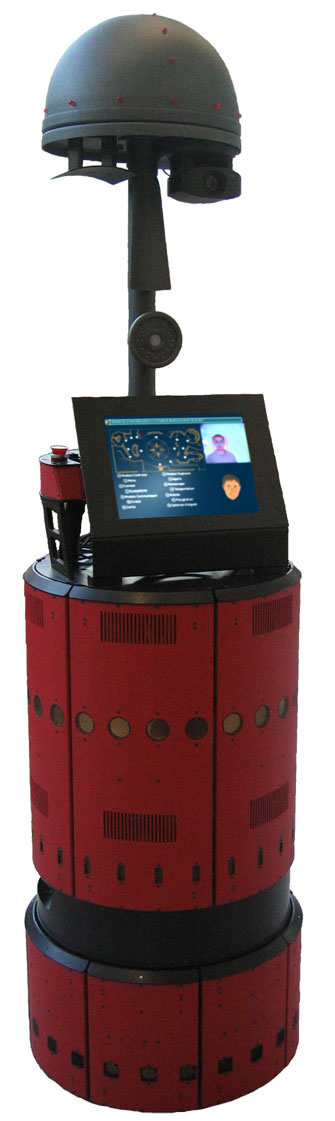
\includegraphics[width=25mm]{rackham.png}}                
  \subfloat[Jido]{\label{fig:Jido}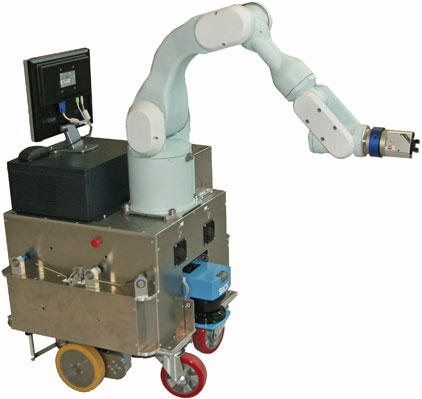
\includegraphics[width=40mm]{jido.png}}
  \subfloat[Dala]{\label{fig:Dala}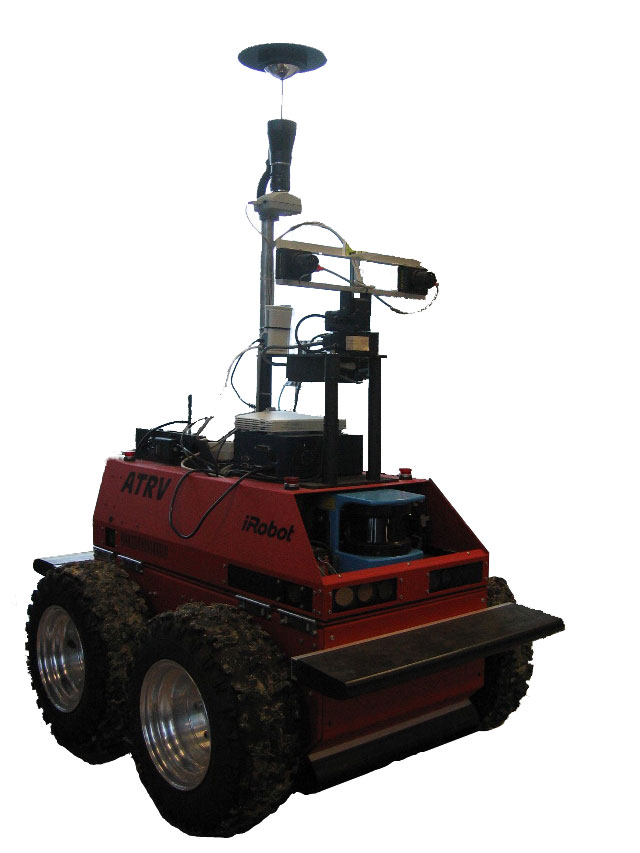
\includegraphics[width=40mm]{dala.png}}
  \caption{LAAS UGVs}
  \label{fig:ugvs}
\end{figure}

\vspace{1cm}

\section{LAAS UAVs}

There have been a number of UAV projects at LAAS: A dirigible named Karma \cite{karma}, and three fixed-wing aircraft: Lhassa \cite{lhassa}, Nirvana, and Manta. The Nirvana aircrafts were used for formation flight \cite{gautier} and not equipped with a sensing payload. Manta, a flying wing with a payload based on commodity X86 hardware, was abandoned due to it's less than convenient size and EMI issues \cite{manta}. These UAVs reuse the autopilot and ground station software and hardware from ENAC's open-source UAV system named paparazzi \cite{paparazzi}.

\section{ELROB competition}

The European Land Robot (ELROB) competition is held yearly in Belgium, and the theme alternates every year between military and civilian \cite{elrob}. For the 2011 civilian event to be held in June, the competition is divided into four scenarios, namely: Reconnaissance and surveillance, Transport, Camp security, and Autonomous navigation. The primary team goal for our UAV in the competition is to assist the UGV by furnishing traversability information that will aid in the path planning process. The time to reach various waypoints is limited, so locating any potential roadblocks or highly traversable terrain beyond the reaches of the UGV sensors is a potential source for route optimizations.

\chapter{Project Description}

Before the project started, specific sensors and a computer board were selected for evaluation. A fixed-wing airframe was also pre-selected. What remained was integrating all these components together into a working platform. In this chapter the individual components are described.

\section{Payload equipment}

The computing platform selected by the group for the UAV is a low-power embedded system based on the Texas Instrument OMAP3 processor (details in Section \ref{sec:AirborneProcessor}). The Gumstix Overo module \cite{Overo}, on which the OMAP processor resides, provides the capacity to run the Linux operating system with minimal physical dimension and power requirements. 

The sensors selected include the Hokuyo UTM-30LX (Section \ref{Hokuyo}), a scanning laser range finder, a CMOS image sensor (Section \ref{caspa}), and an inertial navigation system (XSens MTIG, Section \ref{MTIG}). Apart from the camera, all these sensors are already used extensively at the LAAS and are supported with custom driver software \cite{robotpkg}. Furthermore, these drivers have already been ported for use with the ARM processor architecture.

\begin{figure}[htb]
  \centering
  \subfloat[Hokuyo UTM-30LX]{\label{fig:hokuyo}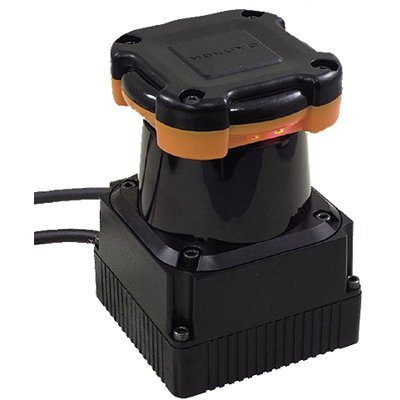
\includegraphics[width=50mm]{hokuyo.jpg}}                
  \subfloat[XSens MTI-G]{\label{fig:mtig}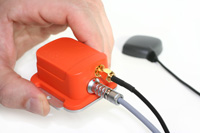
\includegraphics[width=50mm]{MTIG_inhand.jpg}}
  \caption{}
  \label{fig:sensors}
\end{figure}

This payload equipment will reside on-board a low-cost aircraft controlled by the paparazzi autopilot system as detailed in Sections \ref{sec:mentorproject} and \ref{sec:paparazzi}

\section{Airborne Processor}
\label{sec:AirborneProcessor}

In this section we present the miniature embedded computer present on our UAV.

\subsection{Hardware}

The central component of the payload is the Gumstix Overo module (Figure \ref{fig:overo_mod}). The module is used along with a carrier board. The carrier board selected for this project is the Summit product from Gumstix (Figure \ref{fig:overo_summit}). Together, the module and the carrier board contain the TI OMAP processor along with wifi, ethernet, bluetooth transceivers, and a convenient micro SD socket. The TI OMAP System On Chip (SOC) processor incorporates a 600MHz 32-bit ARM Cortex-A8 core, a DSP, and many peripherals including UART, I2C, SPI, SD, USB, and a dedicated camera interface. The package-on-package (POP) configuration, where the SDRAM and NAND memory are stacked directly on top of the processor saves valuable space and weight and decreases EMI/EMC issues. While the camera interface and the DSP provide for future research capabilities, in the near term the important interface is USB Host as this will be used to receive laser scanner data along with other serial-based communications (Inertial Navigation System, ground communication modem, and autopilot communication).

\begin{figure}[htb]
  \centering
  \subfloat[Overo Module]{\label{fig:overo_mod}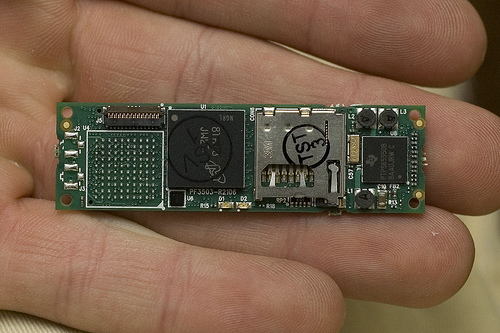
\includegraphics[width=80mm]{overo_in_hand.jpg}}                
  \subfloat[Module on Summit carrier board]{\label{fig:overo_summit}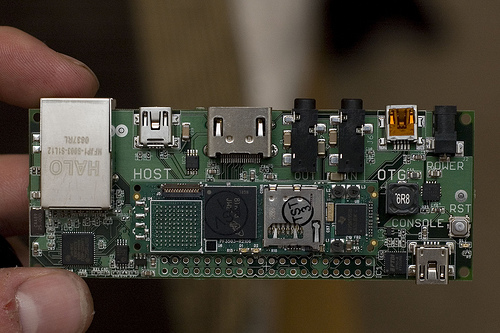
\includegraphics[width=80mm]{overo_on_summit.jpg}}
  \caption{Gumstix Overo}
  \label{fig:overo}
\end{figure}


\subsection{Software}

The OMAP processor runs a full Linux operating system, cross compiled on a standard Linux host using a compilation system called OpenEmbedded. OE is capable of generating the necessary bootloader, linux kernel and modules, along with a root file system populated with all of the libraries and applications that might be needed to run our payload code. Configuration is done using bitbake recipes. With assistance from LAAS developers, bitbake recipes are available for the hokuyo and MTIG device libraries on the OMAP3 plaftorm. These libraries are compiled into ipkg packages that can be installed on the target using the opkg command. Our own custom C++ application links to these libraries and performs all of the acquisition and logging activities. The application is compiled using the paparazzi omap toolchain using a makefile integrated into the paparazzi build environment.

The Makefile and source code are available in Appendix B. To compile the application, use the following paparazzi build command : 

make AIRCRAFT=LASERHAWK getrange.compile

\section{Airborne Sensors}

This section details the miniature sensors carried aloft by our UAV. These include a laser scanner, a camera, and an inertial navigation system.

\subsection{Hokuyo UTM-30LX}
\label{Hokuyo}

The UTM-30LX scans a single line around it's central axis at a maximum rate of 40 Hz. A distance and reflectivity measurement is taken at a resolution of 1/4 of a degree, it's field of vision is 270 degrees, and distance resolution is in the sub-centimeter range. The USB interface, along with open-source software drivers \cite{robotpkg}, allows easy interfacing with PC and embedded hosts, but a number of practical limitations cause the actual maximum data rate to be considerably below what is expected (see results/problems section).

\subsection{Aptina MT9V032 Camera}
\label{caspa}

The MT9V032 CMOS device from Aptina was selected due to its global shutter characteristic that guarantees that all pixels in a frame are acquired simultaneously (unlike the much more common rolling shutter cameras found in most webcams, cell phones, etc). Camera resolution is 752 x 480 pixels and is available in color or black and white. 

The CMOS Camera is interfaced to the OMAP processor using the dedicated camera bus by means of level converters (1.8V/3.3V) and a high-density flat flex cable. This direct connection is a parallel bus with a maximum clock rate of 40MHz, which allows for fast and efficient acquisition of image data. A custom designed camera board using this sensor is in the works at the LAAS while initial testing will depend on the commercially available camera board from Gumstix, INC called Caspapx \cite{caspa}, and displayed in Figure \ref{fig:caspa}.

\begin{figure}[ht]
 \centering
 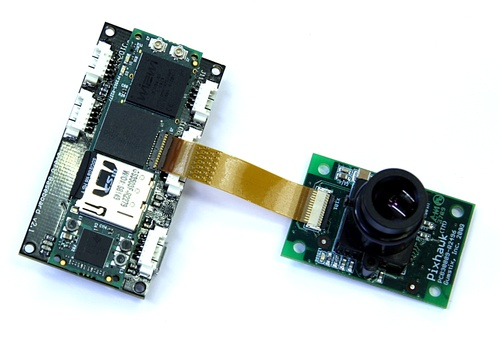
\includegraphics[width=8cm]{overo_and_caspa.jpeg}
 \caption{Overo connected to Caspapx Camera}
 \label{fig:caspa}
\end{figure}

Software support is provided as a linux driver, currently for kernel version 2.6.34. The driver has been tested in flight and performance remains to be determined.

Insert pictures taken in flight here

\subsection{XSens MTIG INS}
\label{MTIG}

The XSens MTIG device uses MEMS sensors along with a GPS receiver to generate attitude and position estimates at a maximum rate of 100Hz using an undocumented Kalman filter running on its embedded processor. It is optionally capable of providing raw sensor measurements at a rate up to 500Hz. The serial interface is well documented and supported with various open-source libraries including LAAS' robotpkg \cite{robotpkg}.


\section{Scan Flight Geometry}
\label{geometry}

The scanner is mounted so that the scan plane is perpendicular to the ground and the aircraft's longitudinal axis. The scan line on the ground is defined by the flight parameters as follows:

nominal UAV flight velocity : 20-30 m/s

nominal UAV flight height AGL : 30 m

Lidar sensor resolution : 1080 points over 270 deg visible (1440 points over 360 deg) @ 40Hz

ground covered distance during one revolution of scanner:
\begin{equation}
Dist_{per\_scan\_rev} = ground\_speed \times time_{per\_scan\_rev} = 20~\frac{m}{s} \times \frac{1}{40}~s = 0.5~m 
\end{equation}

For 90 \degree; interest zone :

scan line advances down ground track :

\begin{equation} 
Dist_{x}=  \frac{90}{360} \times Dist_{per\_scan\_rev} = \frac{1}{4} \times 0.5~m = 12.5~cm
\end{equation}

scan line proceeds along sensor rotation (for a 90 scan, this is twice the AGL height) :

\begin{equation} 
Dist_{y}=  2 \times AGL = 2 \times 30~m = 60~m
\end{equation}

Resolution :

\begin{equation}  
\frac{ \frac{90}{360} \times 1440~pixels }{scan\_length} = 
\frac{360~pixels}{\sqrt{{Dist_x}^2+{Dist_y}^2}} \approx \frac{360~pixels}{Dist_y}= 6~ \frac{pixels}{m} = 17~cm
\end{equation}

Angle relative to track : (negligible relative to crab angle)
\begin{equation} Angle_{scan\_to\_track} = \tan^{-1} \frac{Dist_x}{Dist_y} = \tan^{-1} \frac{0.125}{60} = 0.119^\circ
\end{equation}

This information is sumarized in figure \ref{fig:geo1} and \ref{fig:geo2} below.

\begin{figure}[ht]
  \centering
  \subfloat[Overview]{\label{fig:geo1}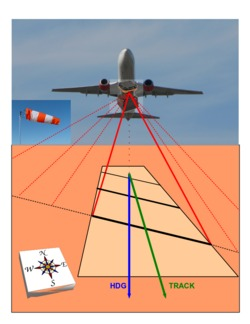
\includegraphics[width=90mm]{geo1.jpg}}                
  \subfloat[Detail]{\label{fig:geo2}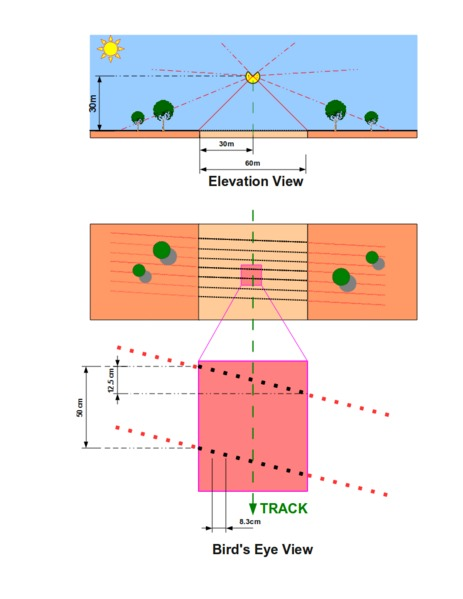
\includegraphics[width=90mm]{geo2.jpg}}
  \caption{Scan Geometry}
  \label{fig:geometry}
\end{figure}

\section{Autopilot System}
\label{sec:paparazzi}

In this section we cover the background information on the open-source UAV platform known as paparazzi. We use this platform in our project to gain an autopilot and a ground station.

\subsection{Paparazzi Description}

Paparazzi is an autopilot system based on a C-code mainloop program running on an airborne ARM microcontroller and Ocaml ground-station code running on a standard Linux PC or laptop \cite{paparazzi}. The system allows for extensive customization and extensions. For example, the flight plan mechanism allows the creation of complex trajectories based on waypoints and conditions. Some other options include support for multiple simultaneous aircraft and ground stations,  a software bus model that makes the creation and insertion of additional software agents into the system straightforward, and various simulation capabilities that are useful in initial testing of code and configurations. Ground to air communications are typically achieved with low-bandwidth serial modems and commercial R/C control receivers and transmitters. 

\subsection{Aircraft Types}

Paparazzi supports fixed-wing and rotating-wing aircraft. There is much recent use on quadrotor platforms, especially the Asctec airframe \cite{asctec}, but helicopter use has so far been very limited. Users of the fixed-wing configuration typically use small foam airframes such as the ones manufactured by RC manufacturer Mutliplex \cite{multiplex}, brushless electric motors, and the wingspans remain below 1.5m. In a few cases, the airframes are much larger, or much smaller, or more complex. These might incorporate fiberglass or carbon airframes for extended runtime \cite{murat} or range \cite{corsica}, or a gas turbine to achieve higher velocities, or larger wing areas and increased payload capacity. Essentially, the PID algorithms implemented in paparazzi are such that just about any standard craft can be controlled if the gains are adjusted properly.

In the most basic and most widely used fixed-wing configuration, the autopilot uses GPS and IR sensors for attitude and navigational control \cite{paparazzi_paper}. Due to some of the drawbacks of these sensors, support for replacement or complimentary sensors exists and is continuously explored. This includes the use of static and dynamic pressure sensing (to allow the aircraft to respect air-speed or altitude bounds or set-points, for example), the use of inertial measurement units (to eliminate the need for a minimum ground/sky IR contrast, for example), and the use of a magnetometer to obtain a measure of the aircraft's heading. To maintain an accurate state estimate with small craft capable of high roll rates, the bandwidth-limited IR sensors are complemented with a roll gyro. This is typically a low-cost MEMS sensor, of the likes from Analog Devices, and interfaced via the autopilot's extra digital interfaces or sampled by an ADC channel.

\subsection{Hardware}

The current autopilot hardware is the Tiny2.1, a 50-gram board with a NXP LPC2148 microcontroller, a U-blox GPS receiver module and antenna, and small Molex Picoblade connectors for interfacing with the following devices :

\begin{itemize}
\item UART-based modem (typically Digi XBee/XBee Pro, or Aerocomm)
\item PPM-based RC receiver input (PPM signal requires receiver modification so certain users have put the effort into using serial-protocol based 2.4GHz receivers)
\item PWM-based RC servo outputs
\item USB for programming by PC Host
\item ADC inputs to sample IR sensors and monitor battery level
\item I2C and SPI interfaces for additional communication, sensor, or actuator options (see examples cited above)
\end{itemize}

\subsection{Paparazzi tradeoffs}

A typical useful hardware and software system must wrestle with the complexity trade-off. Either designs follow the KISS principle, and favor lightweight and easy to master architectures, or they aim to deliver a high degree of modularity and configurability to enable extensibility, continuous reuse and evolution. Paparazzi adopts the KISS principle for hardware designs, choosing to use COTS modules and skipping any redundancy, subscribing to the idea that a simple, straightforward, clean, and well-documented design can be relatively robust and enables a larger community (for many, a hobby activity). The software side is very different because extensibility and configurability were goals from the outset and development has continuously evolved without any milestones or official releases. This has results in a complex and sparsely documented code base that can seem unwieldy to anyone except a dedicated developer with the proper amount of pre-requisite competencies.

Like all active complex configurable systems, the challenge with paparazzi is its steep learning curve and rapid and continuous evolution. Tailoring the system for a specific application is not difficult because paparazzi requires extensive modifications, but because much of the system has to be mastered before a clear idea emerges of how and where the modifications should be made. Since documentation is limited to unstructured wiki pages and due to a complete lack in code comments, a user is essentially forced to become a developer and to dive deep into the system or resort to hacks to limit the time invested. Beyond the obvious drawbacks of the later option, is the fact that such hacks are only useful in the very short-term. Since the hacks will not be able to be merged with the software base, as the base evolves the hacks will continuously break and require constant effort to keep them working. This pressure is the reason why many users have forked the paparazzi code, added their extensive application-specific modifications without staying up to date, to end up with a system that is nearly un-mergeable with the evolved paparazzi code base. The bottom-line is that tailoring paparazzi for a project should be approached in one of two ways depending on the objectives. One, if the intent is to produce a one-off demo and future reuse is not a consideration, a fork can be considered along with quick hacks. If the continuous evolution of the application is envisioned or if sharing the capabilities with other paparazzi users is desired, the time to properly integrate customizations and continuously maintain them needs to be anticipated and allocated. This is the same sort of commitment already in place for the LAAS' openrobots software.

All this to say that considerable time is required integrate paparazzi in any project and that new team members will not able to contribute for the few months it takes to get to know the system.

\chapter{Ground-based Testing}

In an attempt to gain some practical experience, flesh out any early limitations, and begin developing data processing software, a simple ground-based test was carried out.

\section{Test Description}

\begin{figure}[ht]
 \centering
 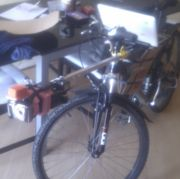
\includegraphics[width=6cm]{Bikesciencepackage.jpg}
 \caption{Bike Test Vehicle}
 \label{fig:bike}
\end{figure}

The hokuyo sensor and the MTIG were mounted on boom attached to a standard bicycle as show in Figure \ref{fig:bike}. While the bicycle traveled through a residential neighborhood, a small laptop logged the sensor data to files. These files show that on a sunny day the hokuyo can detect at a light-colored perpendicular surface up to 20 meters away. UAV testing (discussed later in Section \ref{flight_tests}) will be necessary to determine performance on surfaces such as dirt and grass and at angles approaching 30 to 45 degrees from perpendicular.

\section{Output Sample}

Using a number of PERL programs listed in Appendix B, a composite image is generated including a number of text data such as the MTIG output angles and a graphical representations of laser scan data, the location data, and video taken by a boom mounted digital camera (Figure \ref{fig:plotlogsample}). The images are then put together to create an animation showing the data along the entire path. The hokuyo data was recorded at a rate of approximately 20 Hz while the MTIG Data was near 100Hz. Rough synchronization is accomplished by using the MTIG data sample with a timestamp closest to the one in a laser scan (each laser scan is also timestamped). 

\begin{figure}[ht]
 \centering
 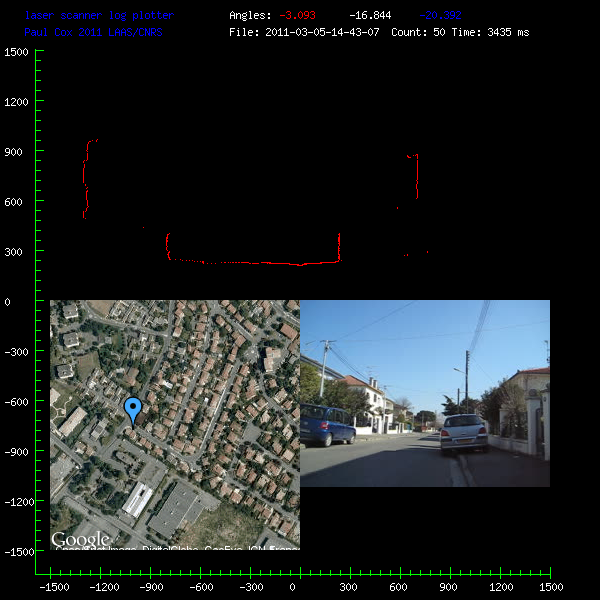
\includegraphics[width=12cm]{Plotlogsample.png}
 \caption{Sample animation frame}
 \label{fig:plotlogsample}
\end{figure}

Ground testing showed the hokuyo device can be used in an exterior setting and that distances of up to 16 meters can be detected even in bright sunlight if the reflecting surface is perpendicular and of a light color.

\section{Post Processing}

The next step is to represent the laser scans in a 3D environment, creating a Digital Terrain Model and representing graphically in an openGL tool such as GDHE. This process can be accomplished with the LAAS tools robotpkg and Jafar, and I am still trying to learn these so this tasks is not yet complete. To become accustomed to these tools and understand the methods behind them, I've developed various applications to work through data acquisition, generation, and processing. The code is available freely online \cite{laserhawkgit}. Some screenshots of these applications are shown below in Figure \ref{fig:mkvirt} and \ref{fig:hoku2gdhe}.

\subsection{Virtual Terrain Generation}

Using the PERL language, I created software that could create sensor logs using a virtual environment. The environment includes a bounded surface that defines the terrain topography and camera orientation. The model can be defined as piece-wise functions or by a greyscale bitmap. An example terrain is shown in Figure \ref{fig:mkvirt}. Lighter colored pixels have higher elevation than darker ones.

\begin{figure}[ht]
 \centering
 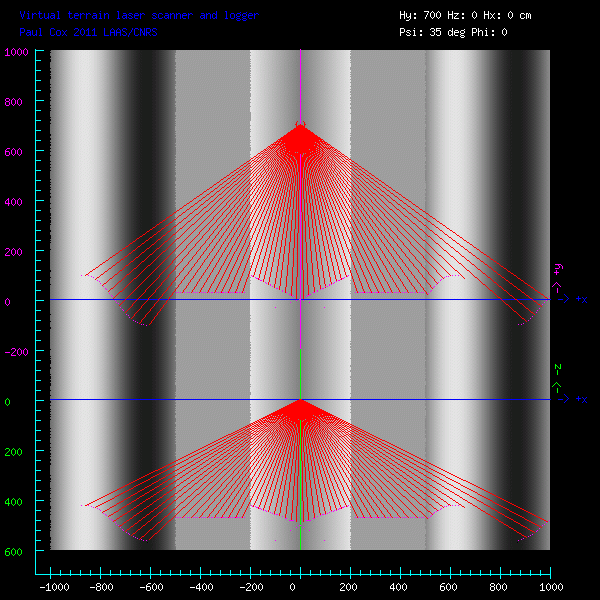
\includegraphics[width=12cm]{Mkvirtsample.png}
 % Mkvirtsample.png: 0x0 pixel, 300dpi, 0.00x0.00 cm, bb=
 \caption{Virtual terrain simulator}
 \label{fig:mkvirt}
\end{figure}

The virtual terrain surface is ``scanned'' along a line by using a raycasting method. Essentially, iterating through the scan angles one step of resolution at a time, the distance between the ``camera`` and the surface is calculated. The calculation is performed by propagating the ray until intersection is detected, and uses some trigonometry to arrive at a final distance (See Figure x).

Insert calculation figure here.

After acquisition of the virtual scan lines into log files, 3D plotting tools can be used to visualize them (Figure \ref{fig:hoku2gdhe})

\subsection{3D Plots of Acquired Virtual Terrain Data}

\begin{figure}[ht]
 \centering
 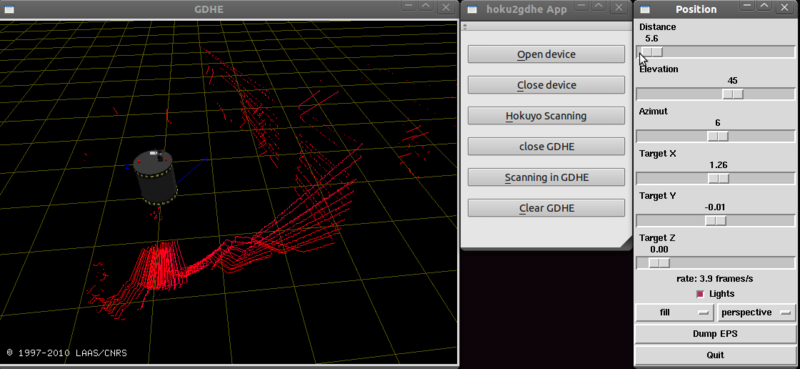
\includegraphics[width=12cm]{Hoku2gdhe.png}
 % Hoku2gdhe.png: 0x0 pixel, 300dpi, 0.00x0.00 cm, bb=
 \caption{Data visualisation in GDHE}
 \label{fig:hoku2gdhe}
\end{figure}


\chapter{Mentor Aircraft Project}
\label{sec:mentorproject}

As explained above, the immediate goal is to outfit a Multiplex Mentor aircraft with a Hokuyo, Gumstix Overo, and MTIG for the June 2011 competition. Towards this goal, I've integrated a paparazzi autopilot in a standard Mentor airframe. I've also built a reinforced modular payload pod to hold the science package in an easy removable format. This permits development with the science package in a lab environment without being encumbered by the airplane, and provides some level of protection in the event of a crash.

\section{Airframe}

The aircraft is a standard three-axis electric R/C model and is displayed in Figure \ref{fig:mentor}. It uses two ailerons, an elevator, and a rudder for control surfaces along with a fourth channel for thrust control.

\begin{figure}[ht]
 \centering
 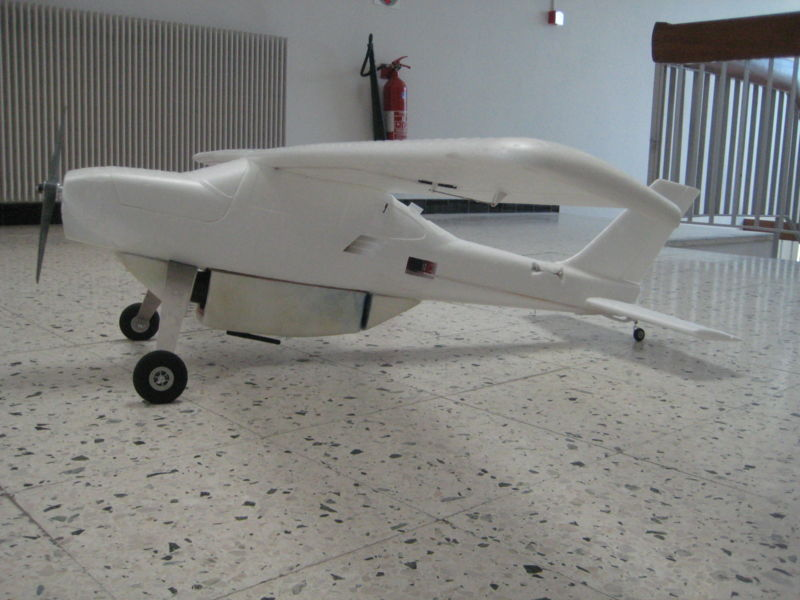
\includegraphics[width=10cm]{800px-Mentor1_2.jpg}
 % 800px-Mentor1_2.jpg: 800x600 pixel, 180dpi, 11.29x8.47 cm, bb=0 0 320 240
 \caption{Completed Mentor Aircraft with Payload}
 \label{fig:mentor}
\end{figure}

The major aircraft components are listed below:

\begin{itemize}
 \item Motor : AXI 2820 Gold Brushless DC
 \item Propellor : APC 10 x 8 ? 
 \item Electronic Speed Controller : 80 Amp Brushless ?
 \item Batteries : 3 series elements Lithium Polymer
 \item RC Receiver : ?
 \item RC Transmitter : ? 
 \item Autopilot: Tiny v1.1 with Ublox LEA-4H GPS receiver
 \item Attitude Sensors : Infrared (6 orthogonal pixels paparazzi analog design)
\end{itemize}

Power for the RC Servos is supplied by an stand-alone BEC (Battery Elimination Circuit) instead of using the power provided by the autopilot board. This is done to eliminate the possibility of power supply rail fluctuations due to the intermittent high current loads generated by the servos. The fluctuations can lead to the autopilot's processor rebooting in flight which can have dire consequences.

Insert close up of autopilot board in airframe.

Insert close up of IR sensors.

\subsection{Airframe Parameters}

The airframe is characterized by a number of traits that must be provided to the autopilot. These characteristics such as minimum and maximum speed, control loop gains, servo ordering and positions, etc, are listed in an xml configuration file in the Appendix (\ref{appendix}). Much of the initial flight testing is aimed at finding adequate gains to achieve tight control and navigation while maintaining stability in a variety of outdoor conditions.

\section{Payload}

The payload pod is built using typical model construction techniques. As seen in Figure \ref{fig:payload}, a plywood frame houses the various components and a glass-fiber reinforced foam cover provides a streamlined shape and protects the pod contents in the event of a crash. The payload is designed for quick insertion and removal from the aircraft, with a single magnetically-held carbon rob used to secure it to the craft. The payload weight is 650 grams and requires the Mentor to fly at higher than normal cruising speeds to generate the necessary lift. 

\begin{figure}[ht]
 \centering
 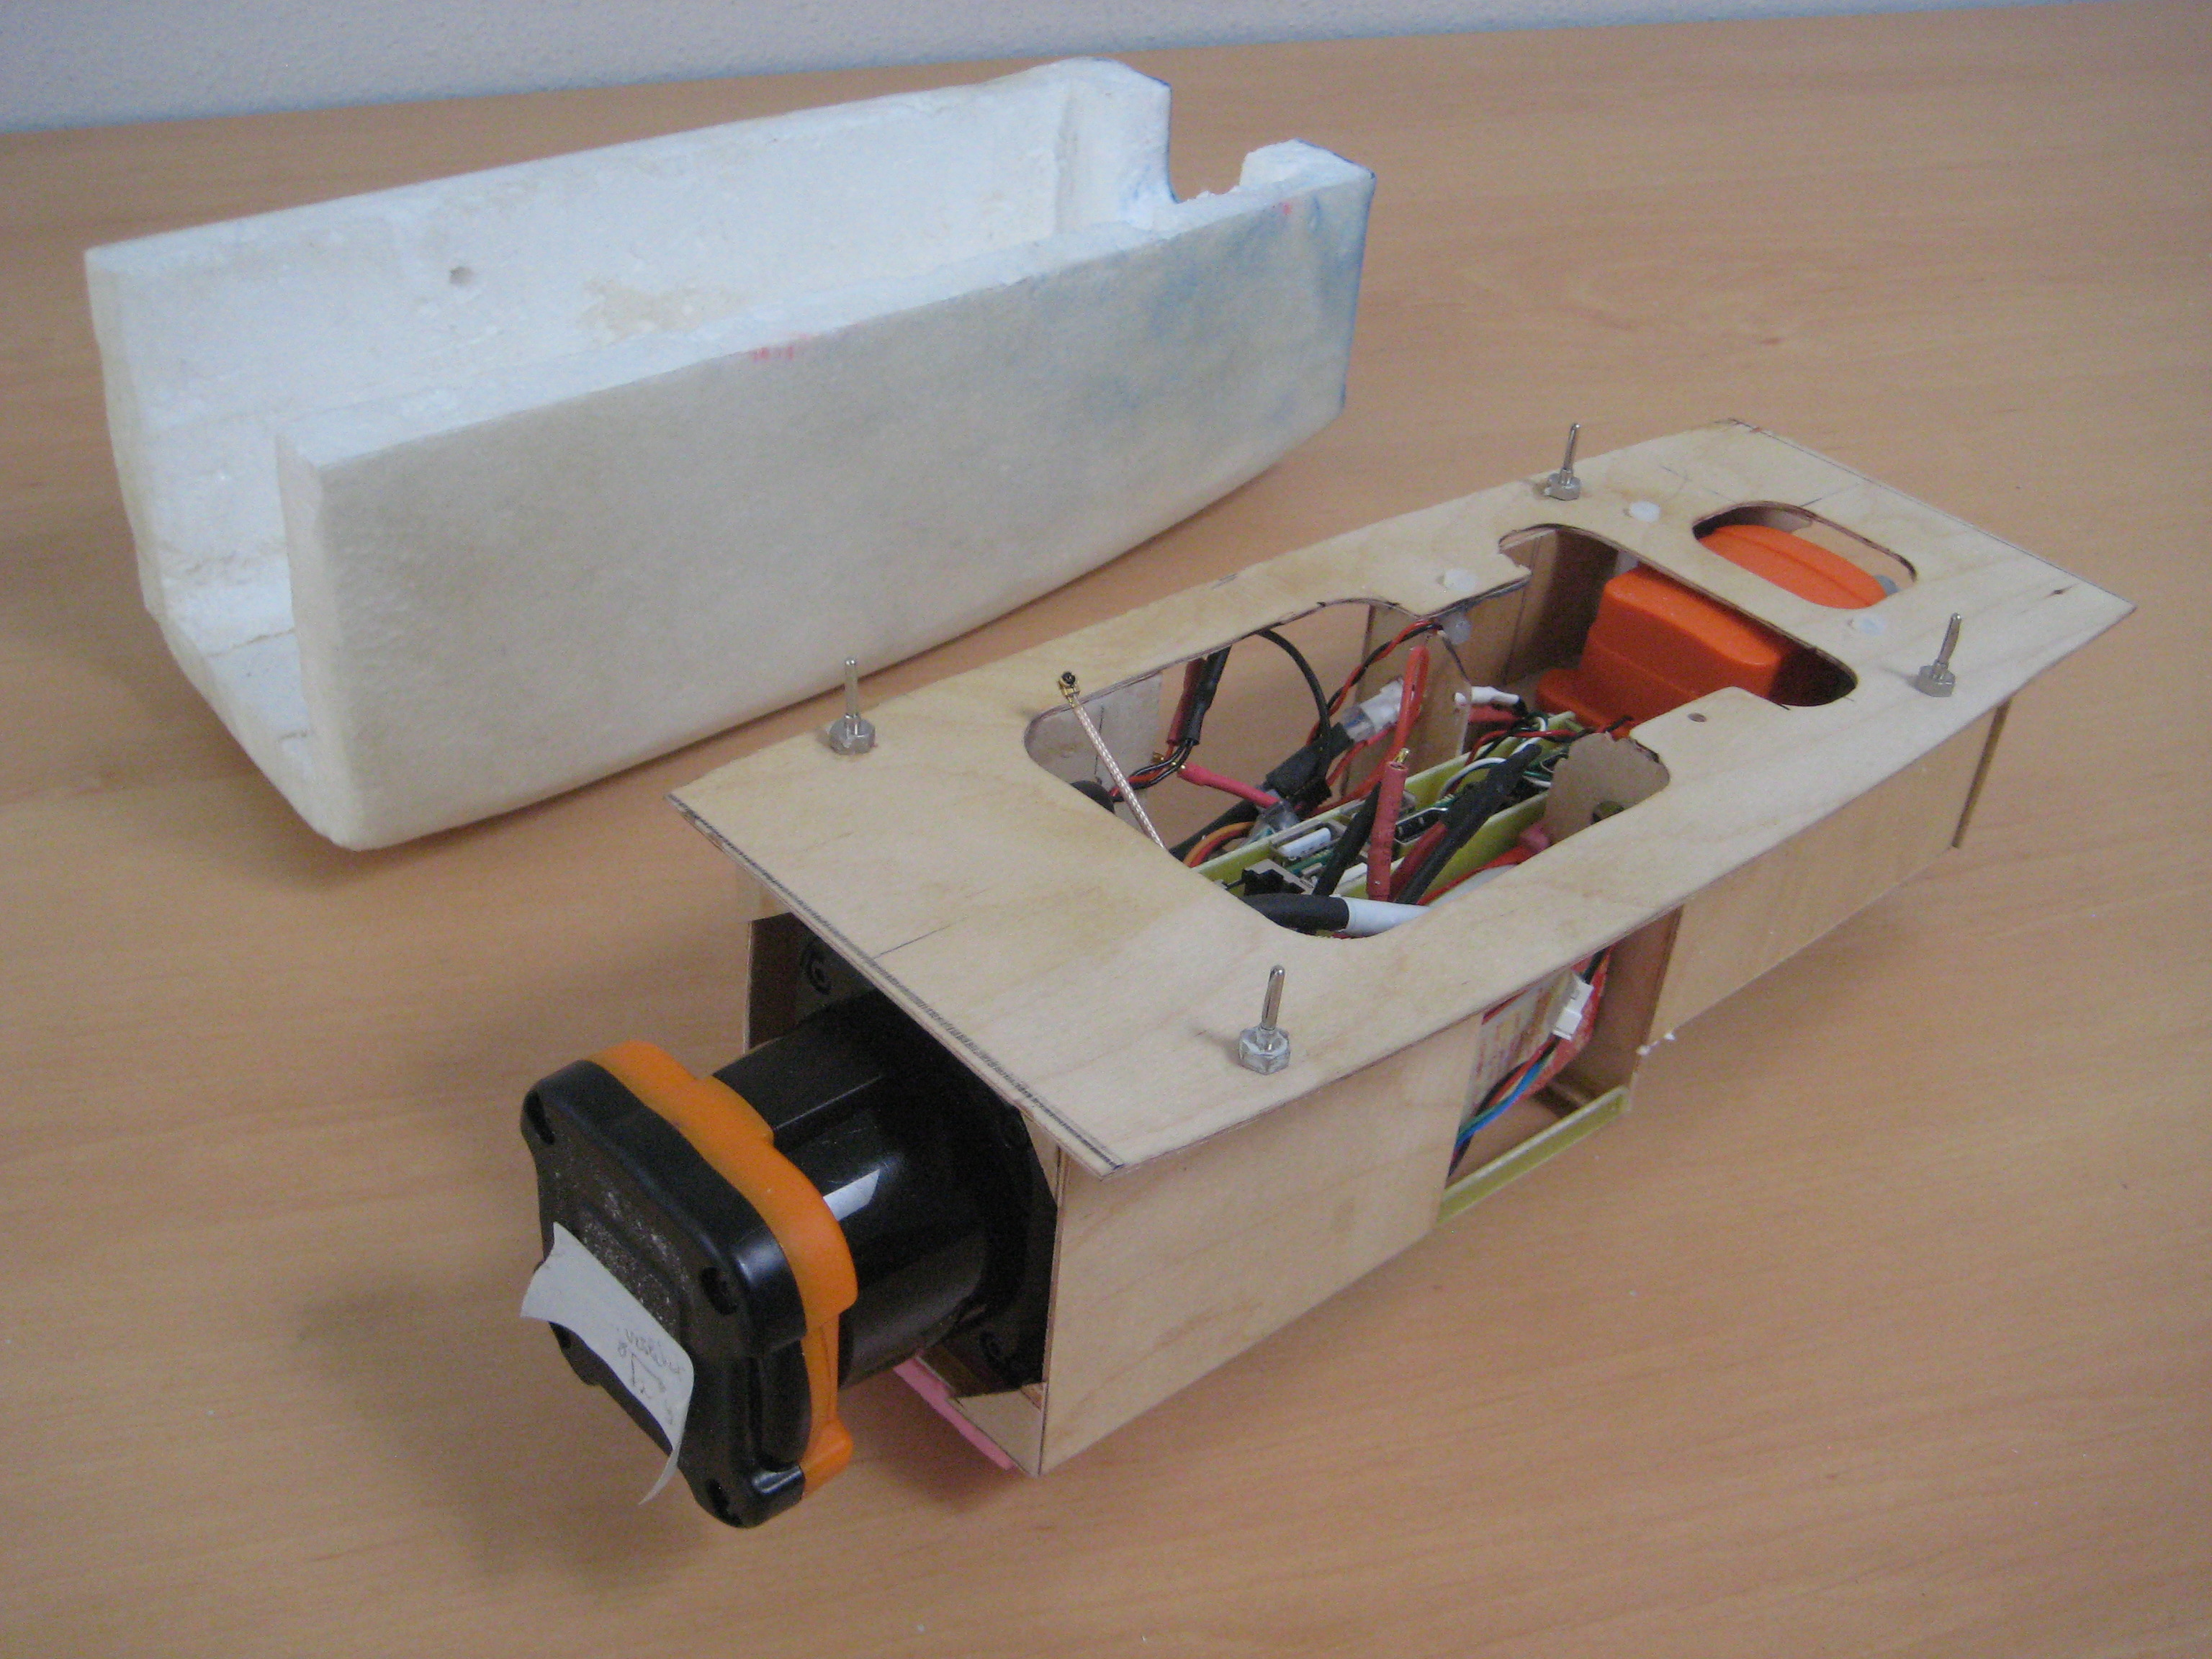
\includegraphics[width=12cm]{Mentor1_payload2.jpg}
 % Mentor1_payload2.jpg: 3072x2304 pixel, 180dpi, 43.35x32.51 cm, bb=0 0 1229 922
 \caption{Completed Payload Pod}
 \label{fig:payload}
\end{figure}

\subsection{Autopilot to Payload interface}

There is a shared ground and two signal connections between the autopilot and the payload.

Since the payload is powered by it's own independent battery, a connection to the autopilot is necessary to allow for monitoring the voltage level. To this end, a voltage divider in the payload provides an output voltage compatible with the autopilot's ADC, and it is connected to a spare input channel on the autopilot board. The voltage level is sent to the ground station as an ADC\_GENERIC message and monitored directly by the ground control user by means of a paparazzi GCS papget (see figure ?). The papget automatically does the conversion from raw ADC value to voltage reading.

insert papget picture here

The second connections between the autopilot and the payload is that the autopilot's telemetry transmit output so that all raw traffic can be logged by the payload. The data is already logged on the paparazzi ground station, but this connection allows the payload to identify where in the cartography flight plan the aircraft currently is, which is useful for knowing when and how to capture and log most efficiently.

\subsection{Block Diagram}

The payload electronics hardware is connected according to Figure \ref{fig:hwdiagram} below.

\begin{figure}[ht]
 \centering
 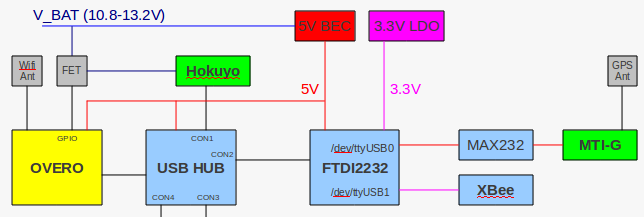
\includegraphics[width=10cm]{payload_hardware_block_diagram.png}
 % Payload_hw_block_diagram.png: 0x0 pixel, 300dpi, 0.00x0.00 cm, bb=
 \caption{Payload Hardware Block Diagram}
 \label{fig:hwdiagram}
\end{figure}

\subsection{Weights}

The weight of the individual components are listed in Figure \ref{fig:weight1} and \ref{fig:weight2}.

\begin{figure}[ht]
  \centering
  \subfloat[Payload]{\label{fig:weight1}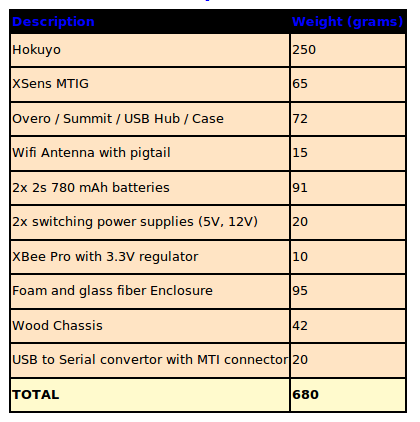
\includegraphics[width=70mm]{weights.png}}                
  \subfloat[Overall]{\label{fig:weight2}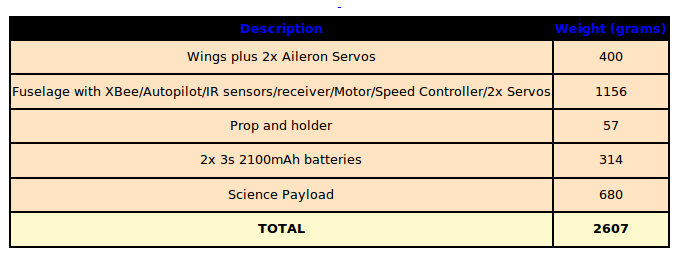
\includegraphics[width=105mm]{weights_overall.png}}
  \caption{Aircraft Weights}
  \label{fig:weights}
\end{figure} 

\section{Cartography Flight Plan}

To request the UAV to fly in parallel tracks above a region of interest, we created a custom flight plan and merged it into the paparazzi source code base. The function allows a region of interest to be defined either before or in flight by the GCS operator by defining three waypoints. These waypoints define a rectangle and the autopilot calculates two sets of parallel tracks, each set perpendicular to the other. The aircraft then flies along these tracks as best as possible given wind conditions and other challenges. Figure \ref{fig:gridcarto} shows the cartography function in action. In the figure, the aircraft can be seen near the center of the image traversing the current ground track highlighted in green. The aircraft track in blue shows the UAVs trajectory since the start of the pattern. The region of interest is defined by the waypoints named S1, S2, S3, and S4, and the tracks within the region are all straight lines.

\begin{figure}[ht]
 \centering
 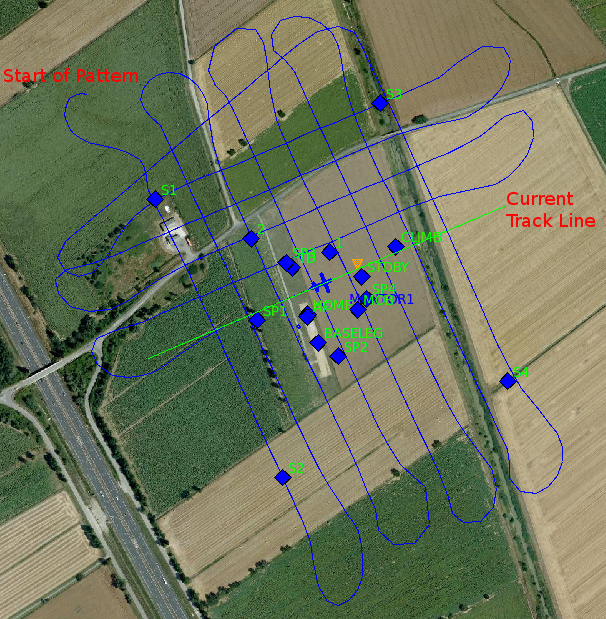
\includegraphics[width=10cm]{pprz_cartography.png}
 \caption{Grid Cartography Flight Plan}
 \label{fig:gridcarto}
\end{figure}

The current cartography function assumes a constant altitude during the entire pattern. Due to the limited laser scanner range of 15-20 meters, this method would only work in relatively flat terrains and without large (>10 meters) obstacles.

\chapter{Flight Testing}
\label{flight_tests}

Flight testing was performed at a small model airfield on the southern outskirts of Toulouse. The site is situation in the midst of wheat fields. There is a small covered work area on site and a row of medium-sized trees. Less than 200 meters away is an irrigation ditch, a road bridge, and some small warehouse buildings.

\begin{figure}[ht]
 \centering
 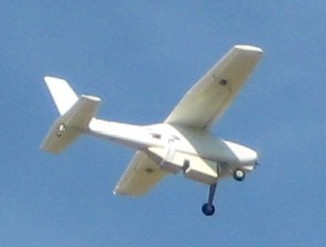
\includegraphics[width=10cm]{mentor_in_flight.JPG}
 % 800px-Mentor1_2.jpg: 800x600 pixel, 180dpi, 11.29x8.47 cm, bb=0 0 320 240
 \caption{Mentor and Payload in Flight}
 \label{fig:mentor_flying}
\end{figure}


\chapter{Challenges}

\section{Hokuyo Lidar performance}

\subsection{Limited lidar range}

Using test flight data, the ability of the lidar sensor to detect the distance to the ground surface was determined by plotting the number of echoes detected for varying aircraft altitudes. The resulting plot as seen in Figure \ref{fig:lidar_perf} shows the inability to detect all echoes starts at an altitude of 9 meters. The number of echoes received in the 90 degree scan region should be 360 as the resolution is four points per degree. Assuming the aircraft is horizontal, the 360 points represent the terrain profile along the scan path whose length is 2x the altitude. So, at 10 meters altitude we are imaging 20 meter swaths (Figure \ref{fig:lidar_scan}). At 15 meters altitude, due to the sensor range limitations, the swaths imaged are much narrower than expected, in the 6 to 9 meter range (Figure \ref{fig:lidar_scan2}).

This test was done in a favorably cloudy day. Performance on a clear day is presumed to be inferior.

\begin{figure}[ht]
 \centering
 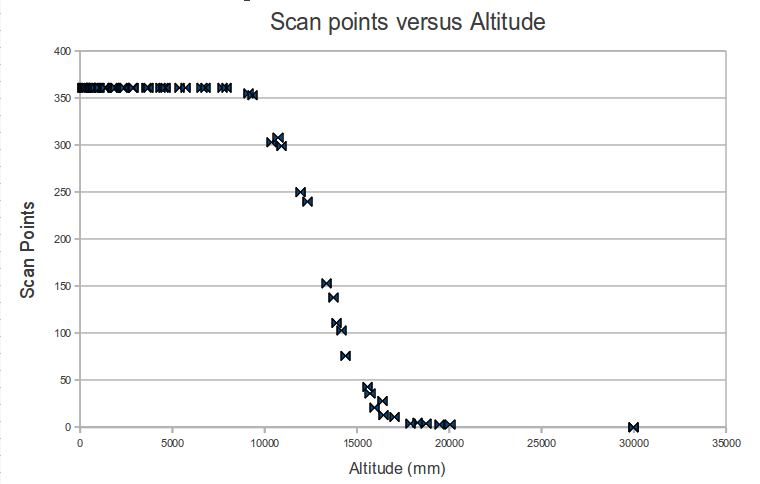
\includegraphics[width=12cm]{scanpt_v_alt.png}
 \caption{Lidar Range Performance in Flight}
 \label{fig:lidar_perf}
\end{figure}


\begin{figure}[ht]
 \centering
 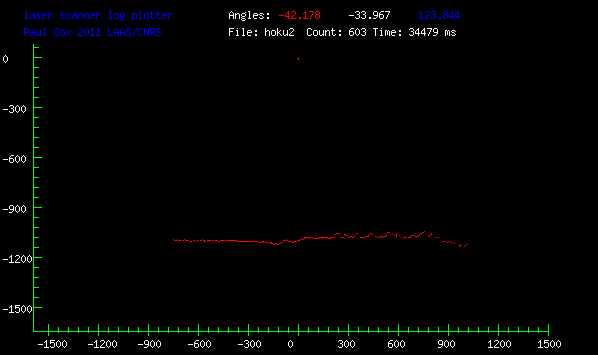
\includegraphics[width=12cm]{scan603.png}
 \caption{Typical Lidar Scan}
 \label{fig:lidar_scan1}
\end{figure}

\begin{figure}[ht]
 \centering
 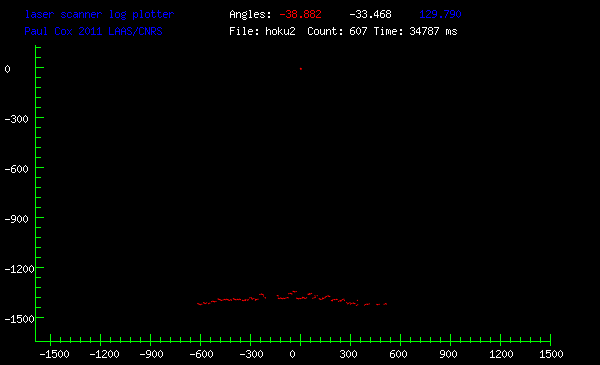
\includegraphics[width=12cm]{scan607.png}
 \caption{Typical Lidar Scan 2}
 \label{fig:lidar_scan2}
\end{figure}

\subsection{Lidar driver limitations}

Transferring the 1081 scan points at 40 scans per second requires considerable CPU time by the scanner driver. If the system is busy with other tasks such as writing to logs, or the compression and transfer of data to the ground station, the processor can be preempted and scans are lost as there is no scan buffering. Also, the scan intensity data is available but it's use leads to a 3-fold decrease in the effective scan rate and is therefor not usable. Finally, a multi-echo feature in the driver appears to only be possible with a different Hokuyo product.

\section{GPS}

Initial testing showed an issue with the buffering of MTIG data. Much of the data was in clumps and the GPS position did not closely follow what was provided by the autopilot. Figure \ref{fig:track_comp} shows a comparison of GPS track recorded with the autopilot and the payload.

\begin{figure}[ht]
  \centering
  \subfloat[Autopilot GPS]{\label{fig:ap_gps}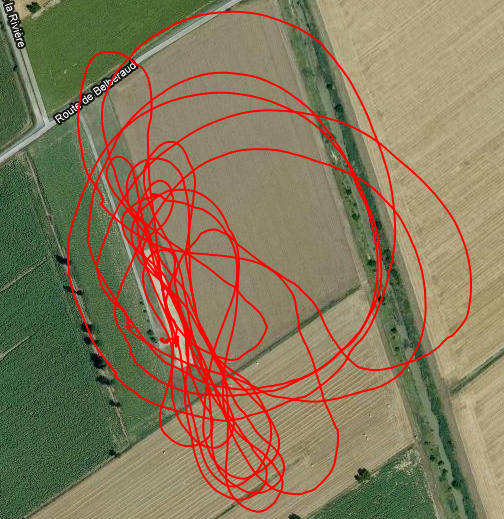
\includegraphics[width=70mm]{11_05_26__17_08_52_pprz_gmap.png}}                
%  \subfloat[Payload GPS]{\label{fig:payload_gps}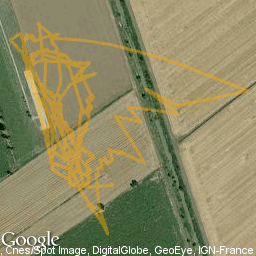
\includegraphics[width=70mm]{hoku2_2000_10000.jpg}}
  \subfloat[Payload GPS]{\label{fig:payload_gps}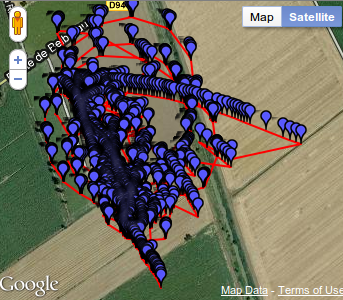
\includegraphics[width=82mm]{hoku2_flight_payload_gps.png}}
  \caption{GPS Tracks}
  \label{fig:track_comp}
\end{figure} 

After some time working with the device driver library it was discovered to be a problem in its use. The problem caused much of the sent data to be lost, the timestamps to not reflect correct acquisition time, and high CPU utilization. 

\section{Time Synchronization of Sensors}
 
Currently there is loose time synchronization based on timestamps added to the scan and INS data streams at the application level. Tighter synchronization is planned in the future by time stamping at a lower level (i.e. in the device drivers) and by hardware sync between the scanner and the camera. The pulse output generated by the scanner at the start of each revolution could be used to trigger the exposure of a camera frame using it's exposure input. This input will be available on the custom camera design currently in development at the LAAS.

\section{Other Challenges}

\begin{itemize}
 \item Limited LIDAR resolution between scan lines at high aircraft velocities.
 \item Maintaining constant Above-Ground-Level (AGL) altitude in varying terrain to stay within the 10-15 m LIDAR range.
 \item Detecting obstacles in the flight path to avoid tree tops, for example.
 \item Accurate attitude and position estimates needed for accurate data correction and geo-referencing.
 \item Limited range on R/C Link (150 m max for low altitudes which is less than ideal)
 \item Limited autonomy due to limited battery capacity (10-12 minutes maximum)
 \item Limited capacity of autopilot to closely follow flight plan tracks (even straight lines) in fluctuating or high winds
 \item Frequent hardware failures due to the low-cost nature of RC products. Servos often die unexpectedly, intermittent solder joints on IR sensors, etc.
\end{itemize}

\chapter{Conclusion and Future Direction}

This project showed that it is possible to fly the requested sensors on an autonomous aircraft. The Lidar was capable of scanning in daylight conditions and this data could be recorded along with relatively accurate attitude and position estimates.

Unfortunately, the limited range of the sensors and autonomy of the aircraft render the UAV useful for only a few potential scenarios. The environment to be scanned must not have elevations that vary more than a few meters and obstacles must also be only a few meters in size. This lends itself well in looking for ditches and roads in a typical desert or agricultural landscapes, but not at all for wooded or urban environments.

Another drawback with the project aircraft was that velocities in the 15 to 20 m/s range and a maximum lidar scan rate of 40 Hz results in large unmapped areas. Future investigations could focus on fusing camera data with the lidar scan data to potentially generate traversability estimates. For example, a downed tree trunk might appear as a round or oval feature in a couple of laser scan lines, and the camera data might show this is a continuous obstacle and define its extents.

By using the laser data to regulate the aircraft's altitude, it would be possible to follow gently changing terrain elevations. Another possibility worth investigation is the deflection of part or parts of the hokuyo's 270 degree scanning range towards the front of the aircraft. These scan portions could be used to detect obstacles and instruct the autopilot to fly over or around them, although the limited lidar range and high aircraft velocities would seriously limit this capability.

By using a different lidar scanner or improving the current driver performance, it would also be interesting to be able to receive intensity and multi-echo data. This data is useful for constructing terrain models in the presence of trees with leaves, for example.

Finally, due to the effective 10m lidar range, to stay safely above the terrain and achieve higher scan density, moving to either a slow flying airplane (5-7 m/s) or a quadrotor is required. Designs for these types of craft with payload capacity in the 700 gram range could be constructed at minimal cost.

\begin{thebibliography}{9}

\bibitem{ugvs}
  \url{http://homepages.laas.fr/matthieu/robots/}

%http://spiderman-2.laas.fr/robots/index.php

\bibitem{rackham}
  \url{http://homepages.laas.fr/sara/robots/rackham/index.php}

\bibitem{jido}
  \url{http://homepages.laas.fr/matthieu/robots/jido.shtml}

\bibitem{dala}
  \url{http://homepages.laas.fr/sara/robots/dala/index.php}

\bibitem{this}
  \url{http://paparazzi.enac.fr/wiki/Laserhawk}

\bibitem{karma}
  \url{http://homepages.laas.fr/matthieu/robots/karma.shtml}

\bibitem{lhassa}
  \url{http://homepages.laas.fr/sara/robots/lhassa/index.php}

\bibitem{gautier}
  Gautier Hattenberger,
  \emph{Formation flight: evaluation of autonomous configuration control algorithms}.
  \url{homepages.laas.fr/simon/publis/HATTENBERGER-IAV-2007.pdf}
  Intelligent Robots and Systems, 2007. IROS 2007. IEEE/RSJ International Conference, 
  2007.

\bibitem{manta}
  \url{http://homepages.laas.fr/bvandepo/wiki/doku.php?id=descriptionmanta}

\bibitem{caspa}
  \url{http://wiki.gumstix.org/index.php?title=Caspa_camera_boards}

\bibitem{robotpkg}
  \url{http://www.openrobots.org/wiki}

\bibitem{laserhawkgit}
  \url{https://github.com/paulcox/laserhawk}

\bibitem{paparazzi}
  \url{http://paparazzi.enac.fr/wiki/Main_Page}

\bibitem{elrob}
  \url{http://www.elrob.org/}

\bibitem{omap}
  \url{processors.wiki.ti.com/index.php/OMAP3_Overview}

\bibitem{Overo}
  \url{http://www.gumstix.com/store/catalog/product_info.php?products_id=211}

\bibitem{asctec}
  \url{http://www.asctec.de/home-en}

\bibitem{multiplex}
  \url{http://www.multiplexusa.com/}

\bibitem{murat}
  Murat Bronz, Jean Marc Moschetta, Pascal Brisset, Michel Gorraz
  \emph{Towards a Long Endurance MAV}
  \url{http://www.recherche.enac.fr/LOTA/lib/exe/fetch.php?id=pascal_brisset&cache=cache&media=03-bronz_moschetta_ijmav.pdf}
  \url{www.emav09.org/EMAV-final-papers/paper_78.pdf}
  International Journal of Micro Air Vehicles
  Volume 1 · Number 4 · December 2009

\bibitem{corsica}
  \url{http://paparazzi.enac.fr/wiki/Corsica}

\bibitem{paparazzi_paper}
  Pascal Brisset, Antoine Drouin, Michel Gorraz, Pierre-Selim Huard and Jeremy Tyler
  \emph{The Paparazzi Solution}
  \url{http://www.recherche.enac.fr/paparazzi/papers_2006/mav06_paparazzi.pdf}
  MAV '06,
  October 2006

\end{thebibliography}

\appendix
\appendixpage
\addappheadtotoc

\chapter{Airframe Configuration}

\definecolor{listinggray}{gray}{0.9}
\definecolor{lbcolor}{rgb}{0.9,0.9,0.9}

\lstset{
  basicstyle=40pt,       % the size of the fonts that are used for the code
  numbersep=25pt,
  numbers=left,
  backgroundcolor=\color{lbcolor},
  tabsize=4,
  rulecolor=,
  language=XML,
  basicstyle=\scriptsize,
  upquote=true,
  aboveskip={1.5\baselineskip},
  columns=fixed,
  showstringspaces=false,
  extendedchars=true,
  breaklines=true,
  prebreak = \raisebox{0ex}[0ex][0ex]{\ensuremath{\hookleftarrow}},
  frame=single,
  showtabs=false,
  showspaces=false,
  showstringspaces=false,
  identifierstyle=\ttfamily,
  keywordstyle=\color[rgb]{0,0,1},
  commentstyle=\color[rgb]{0.133,0.545,0.133},
  stringstyle=\color[rgb]{0.627,0.126,0.941},
}

\lstset{caption=Airframe Configuration}

\begin{lstlisting}
<!DOCTYPE airframe SYSTEM "../airframe.dtd">


<airframe name="Mentor Laas N1 Tiny 1.1">


  <firmware name="fixedwing">
    <target name="sim" 			board="pc">
      <define name="AGR_CLIMB" />
      <define name="LOITER_TRIM" />
      <define name="ALT_KALMAN" />
    </target>
    <target name="ap" 			board="tiny_1.1">
      <define name="AGR_CLIMB" />
      <define name="LOITER_TRIM" />
      <define name="ALT_KALMAN" />
    </target>

    <subsystem name="radio_control" type="ppm"/>

    <!-- Communication -->
    <subsystem name="telemetry" 	type="transparent">
      <configure name="MODEM_BAUD" 		value="B57600"/>
    </subsystem>

    <subsystem name="control"/>
    <!-- Sensors -->
    <subsystem name="attitude" 		type="infrared">
      <configure name="ADC_IR1" value="ADC_1"/>
      <configure name="ADC_IR2" value="ADC_0"/>
      <configure name="ADC_IR_TOP" value="ADC_3"/>
    </subsystem>
    <subsystem name="gps" 		    type="ublox_lea4p"/>
    <subsystem name="navigation"/>

  </firmware>

  <firmware name="setup">
    <target name="tunnel"           board="tiny_1.1" />
    <target name="setup_actuators"  board="tiny_1.1" />
  </firmware>

  <modules>
    <load name="cartography.xml"/>
    <load name="adc_generic.xml">
      <configure name="ADC_CHANNEL_GENERIC1" value="ADC_2"/>
      <configure name="ADC_CHANNEL_GENERIC2" value="ADC_4"/>
    </load>
  </modules>

<!-- commands section -->
  <servos>
    <servo name="THROTTLE"   no="0" min="1200" neutral="1200" max="2000"/>
    <servo name="AILERON_LEFT"  no="3" min="1900" neutral="1550" max="1100"/>
    <servo name="AILERON_RIGHT" no="1" min="1900" neutral="1520" max="1100"/>
    <servo name="RUDDER" no="4" min="1850" neutral="1500" max="1150"/>
    <servo name="ELEVATOR" no="5" min="2200" neutral="1400" max="1000"/>
  </servos>

  <commands>
    <axis name="THROTTLE" failsafe_value="0"/>
    <axis name="ROLL"     failsafe_value="0"/>
    <axis name="PITCH"    failsafe_value="0"/>
    <axis name="YAW"      failsafe_value="0"/>
  </commands>

  <rc_commands>
    <set command="THROTTLE" value="@THROTTLE"/>
    <set command="ROLL"     value="@ROLL"/>
    <set command="PITCH"    value="@PITCH"/>
    <set command="YAW"    value="@YAW"/>
  </rc_commands>

  <section name="MIXER">
    <define name="AILERON_DIFF" value="0.66"/>
    <define name="COMBI_SWITCH" value="1.0"/>
  </section>

  <command_laws>
    <set servo="THROTTLE"           value="@THROTTLE"/>
    <set servo="ELEVATOR" value="@PITCH"/>
    <set servo="RUDDER" value="@YAW + @ROLL*COMBI_SWITCH"/>

    <let var="roll" value="@ROLL"/>
    <set servo="AILERON_LEFT" value="($roll > 0 ? 1 : AILERON_DIFF) * $roll"/>
    <set servo="AILERON_RIGHT" value="($roll > 0 ? AILERON_DIFF : 1) * $roll"/>
  </command_laws>

  <section name="AUTO1" prefix="AUTO1_">
    <define name="MAX_ROLL" value="0.6"/>
    <define name="MAX_PITCH" value="0.6"/>
  </section>

  <section name="INFRARED" prefix="IR_">
    <define name="ROLL_NEUTRAL_DEFAULT" value="-2.6" unit="deg"/>
    <define name="PITCH_NEUTRAL_DEFAULT" value="0.6" unit="deg"/>

    <define name="HORIZ_SENSOR_TILTED" value="1"/>
    <define name="IR2_SIGN" value="-1"/>
    <define name="TOP_SIGN" value="-1"/>

    <!--linear name="RollOfIrs" arity="2" coeff1="0.7" coeff2="0.7"/>
    <linear name="PitchOfIrs" arity="2" coeff1="-0.7" coeff2="0.7"/>
    <linear name="TopOfIr" arity="1" coeff1="1.5"/-->

    <define name="ADC_IR1_NEUTRAL" value="507"/>
    <define name="ADC_IR2_NEUTRAL" value="509"/>
    <define name="ADC_TOP_NEUTRAL" value="515"/>

    <define name="LATERAL_CORRECTION" value="1."/>
    <define name="LONGITUDINAL_CORRECTION" value="1."/>
    <define name="VERTICAL_CORRECTION" value="1."/>
  </section>

  <section name="BAT">
    <define name="MILLIAMP_AT_FULL_THROTTLE" value="40000"/>
    <define name="CATASTROPHIC_BAT_LEVEL" value="9.3" unit="V"/>
  </section>

  <section name="MISC">
    <define name="NOMINAL_AIRSPEED" value="18." unit="m/s"/>
    <define name="MINIMUM_AIRSPEED" value="11." unit="m/s"/>
    <define name="MAXIMUM_AIRSPEED" value="33." unit="m/s"/>
    <define name="CARROT" value="3." unit="s"/>
    <define name="KILL_MODE_DISTANCE" value="(1.5*MAX_DIST_FROM_HOME)"/>
<!--    <define name="XBEE_INIT" value="\"ATPL2\rATRN1\rATTT80\rATBD6\rATWR\r\""/> -->
    <define name="XBEE_INIT" value="\"ATPL2\rATRN1\rATTT80\r\""/>
<!--    <define name="NO_XBEE_API_INIT" value="TRUE"/> -->
    <define name="ALT_KALMAN_ENABLED" value="TRUE"/>
    <define name="TRIGGER_DELAY" value="1."/>
    <define name="DEFAULT_CIRCLE_RADIUS" value="80."/>
  </section>

  <section name="VERTICAL CONTROL" prefix="V_CTL_">

    <define name="POWER_CTL_BAT_NOMINAL" value="11.1" unit="volt"/>
    <!-- outer loop proportional gain -->
    <define name="ALTITUDE_PGAIN" value="-0.15"/>
    <!-- outer loop saturation -->
    <define name="ALTITUDE_MAX_CLIMB" value="2."/>

    <!-- auto throttle inner loop -->
    <define name="AUTO_THROTTLE_NOMINAL_CRUISE_THROTTLE" value="0.55"/>
    <define name="AUTO_THROTTLE_MIN_CRUISE_THROTTLE" value="0.30"/>
    <define name="AUTO_THROTTLE_MAX_CRUISE_THROTTLE" value="0.90"/>
    <define name="AUTO_THROTTLE_LOITER_TRIM" value="0"/>
    <define name="AUTO_THROTTLE_DASH_TRIM" value="0"/>
    <define name="AUTO_THROTTLE_CLIMB_THROTTLE_INCREMENT" value="0.05" unit="%/(m/s)"/>
    <define name="AUTO_THROTTLE_PGAIN" value="-0.03"/>
    <define name="AUTO_THROTTLE_IGAIN" value="0.05"/>
    <define name="AUTO_THROTTLE_PITCH_OF_VZ_PGAIN" value="0.03"/>
    
    <!-- auto pitch inner loop -->
    <define name="AUTO_PITCH_PGAIN" value="-0.065"/>
    <define name="AUTO_PITCH_IGAIN" value="0.15"/>
    <define name="AUTO_PITCH_MAX_PITCH" value="0.35"/>
    <define name="AUTO_PITCH_MIN_PITCH" value="-0.35"/>

    <define name="THROTTLE_SLEW" value="0.05"/>

  </section>

  <section name="HORIZONTAL CONTROL" prefix="H_CTL_">
    <define name="COURSE_PGAIN" value="-1."/>
    <define name="ROLL_MAX_SETPOINT" value="0.6" unit="radians"/>
    <define name="PITCH_MAX_SETPOINT" value="0.5" unit="radians"/>
    <define name="PITCH_MIN_SETPOINT" value="-0.5" unit="radians"/>


    <define name="ROLL_ATTITUDE_GAIN" value="-10000"/>
    <define name="AILERON_OF_THROTTLE" value="0.0"/>
    <define name="PITCH_PGAIN" value="-12000."/>
    <define name="PITCH_DGAIN" value="1.5"/>
    <define name="ELEVATOR_OF_ROLL" value="1250"/>
  </section>

  <section name="NAV">
    <define name="NAV_PITCH" value="0."/>
    <define name="NAV_GLIDE_PITCH_TRIM" value="0"/>
    <define name="NAV_GROUND_SPEED_PGAIN" value="-0.015"/>
    <define name="NAV_FOLLOW_PGAIN" value="-0.05"/>
  </section>

  <section name="FORMATION" prefix="FORM_">
    <define name="CARROT" value="3." unit="s"/> <!-- carrot distance for followers -->
    <define name="POS_PGAIN" value="0.02"/> <!-- coef on position error -->
    <define name="SPEED_PGAIN" value="0.4"/> <!-- coef on speed error -->
    <define name="COURSE_PGAIN" value="0.8"/> <!-- coef on course error (override course pgain for followers) -->
    <define name="ALTITUDE_PGAIN" value="0.1"/> <!-- coef on altitude error -->
    <define name="PROX" value="60." unit="m"/> <!-- proximity distance -->
    <define name="MODE" value="0"/> <!-- mode 0 = global, 1 = local -->
  </section>

  <section name="TCAS" prefix="TCAS_">
    <define name="TAU_TA" value="10." unit="s"/> <!-- traffic advisory -->
    <define name="TAU_RA" value="6." unit="s"/> <!-- resolution advisory -->
    <define name="ALIM" value="15." unit="m"/> <!-- altitude limitation -->
    <define name="DT_MAX" value="2000" unit="ms"/> <!-- lost comm or timeout -->
  </section>

  <section name="POTENTIAL">
    <define name="FORCE_POS_GAIN" value="50"/>
    <define name="FORCE_SPEED_GAIN" value="1"/>
    <define name="FORCE_CLIMB_GAIN" value="8"/>
  </section>

  <section name="AGGRESSIVE" prefix="AGR_">
    <define name="BLEND_START" value="20"/><!-- Altitude Error to Initiate Aggressive Climb CANNOT BE ZERO!!-->
    <define name="BLEND_END" value="10"/><!-- Altitude Error to Blend Aggressive to Regular Climb Modes  CANNOT BE ZERO!!-->
    <define name="CLIMB_THROTTLE" value="0.8"/><!-- Gaz for Aggressive Climb -->
    <define name="CLIMB_PITCH" value="0.3"/><!-- Pitch for Aggressive Climb -->
    <define name="DESCENT_THROTTLE" value="0.1"/><!-- Gaz for Aggressive Decent -->
    <define name="DESCENT_PITCH" value="-0.25"/><!-- Pitch for Aggressive Decent -->
    <define name="CLIMB_NAV_RATIO" value="0.8"/><!-- Percent Navigation for Altitude Error Equal to Start Altitude -->
    <define name="DESCENT_NAV_RATIO" value="1.0"/>
  </section>

  <section name="FAILSAFE" prefix="FAILSAFE_">
    <define name="DELAY_WITHOUT_GPS" value="1" unit="s"/>
    <define name="DEFAULT_THROTTLE" value="0.3" unit="%"/>
    <define name="DEFAULT_ROLL" value="0.3" unit="rad"/>
    <define name="DEFAULT_PITCH" value="0.5" unit="rad"/>
    <define name="HOME_RADIUS" value="100" unit="m"/>
  </section>

  <section name="SIMU">
    <define name="YAW_RESPONSE_FACTOR" value="1."/>
  </section>

 <makefile>

  </makefile>
</airframe>
\end{lstlisting}

\chapter{Code Listings}

\lstset{
  basicstyle=40pt,       % the size of the fonts that are used for the code
  numbersep=25pt,
  numbers=left,
  backgroundcolor=\color{lbcolor},
  tabsize=4,
  rulecolor=,
  language=PERL,
  basicstyle=\scriptsize,
  upquote=true,
  aboveskip={1.5\baselineskip},
  columns=fixed,
  showstringspaces=false,
  extendedchars=true,
  breaklines=true,
  prebreak = \raisebox{0ex}[0ex][0ex]{\ensuremath{\hookleftarrow}},
  frame=single,
  showtabs=false,
  showspaces=false,
  showstringspaces=false,
  identifierstyle=\ttfamily,
  keywordstyle=\color[rgb]{0,0,1},
  commentstyle=\color[rgb]{0.133,0.545,0.133},
  stringstyle=\color[rgb]{0.627,0.126,0.941},
}

\lstset{caption=}

\section{mkvirtlog.pl}
\lstinputlisting[]{../log2gdhe/mkvirtlog.pl}
\section{mkvirts.pl}
\lstinputlisting[]{../log2gdhe/mkvirts.pl}
\section{plotlogs.pl}
\lstinputlisting[]{../biketest/scripts/plotlogs.pl}
\section{animatelogs.pl}
\lstinputlisting[]{../biketest/scripts/animatelogs.pl}
\section{getmaps.pl}
\lstinputlisting[]{../biketest/scripts/getmaps.pl}
\section{gmaps.pl}
\lstinputlisting[]{../biketest/scripts/utils/gmaps.pl}
\section{hokumti.pl}
This Perl script runs on the airborne target and uses an early version of the getrange executable to obtain the hokuyo range data and the MTIHardTest executable to obtain the MTI data. Due to high CPU utilization, it was abandoned for the getrange program below which does all data acquisition and logging from within a single application/thread.
\lstinputlisting[]{../biketest/scripts/utils/hokumti.pl}

\lstset{language=C++}
\section{getrange C++ program}
This program runs on the omap target and is responsible for gathering all sensor data, logging it, and sending it to the ground.
\lstinputlisting[]{../../bvdp_pprz/sw/airborne/firmwares/laserhawk/main.cpp}

\lstset{language=make}
\section{Laserhawk.xml}
This is the makefile used to compile getrange.c
\lstinputlisting[]{../../bvdp_pprz/conf/airframes/LAAS/laserhawk.xml}

\end{document}          
